\section{Diagrammes de Séquences}

\begin{figure}[H]
	\begin{center}
		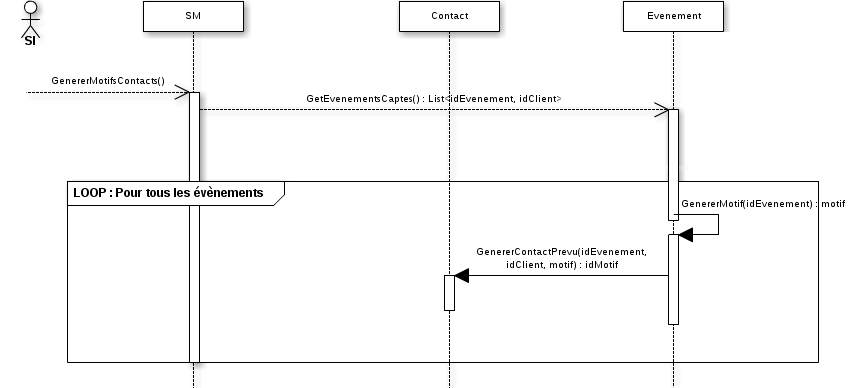
\includegraphics[scale=0.4]{Includes/SOA-Sequence-CU1.png}
		\caption{Diagramme de séquence pour le CU1}
	\end{center}
\end{figure}

\begin{figure}[H]
	\begin{center}
		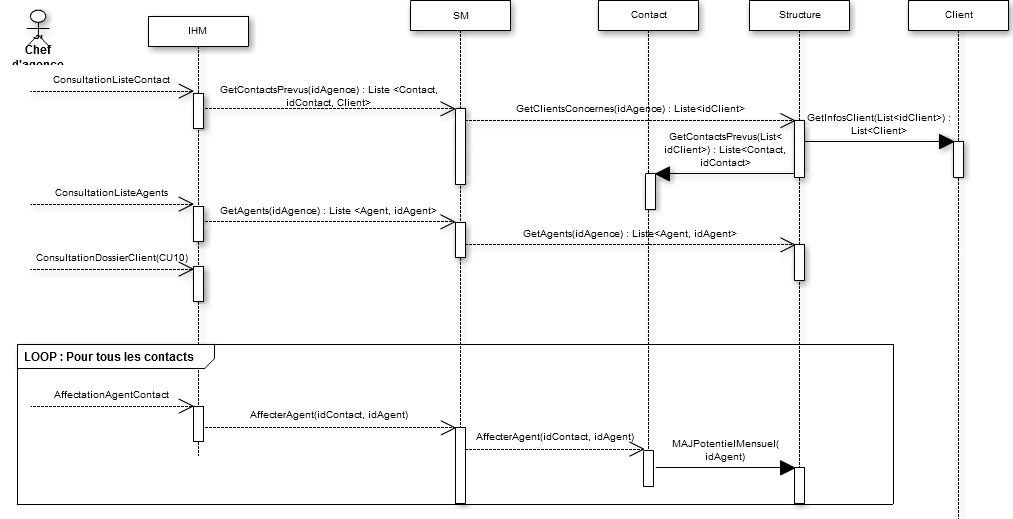
\includegraphics[scale=0.4]{Includes/SOA-Sequence-CU2.png}
		\caption{Diagramme de séquence pour le CU2}
	\end{center}
\end{figure}

\begin{figure}[H]
	\begin{center}
		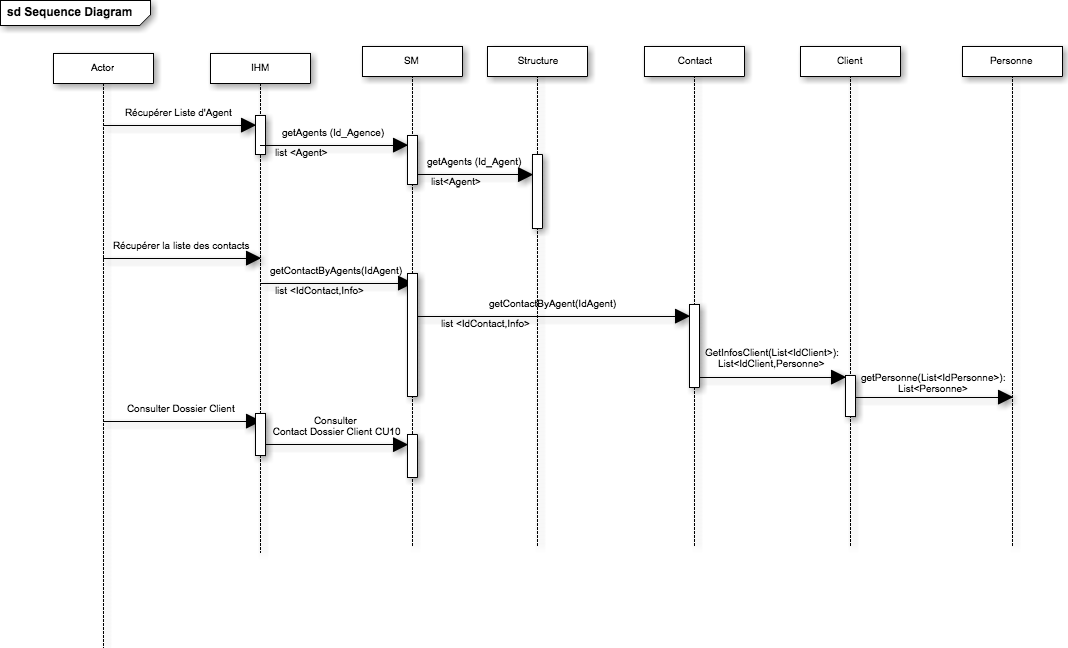
\includegraphics[scale=0.4]{Includes/SOA-Sequence-CU3.png}
		\caption{Diagramme de séquence pour le CU3}
	\end{center}
\end{figure}

\begin{figure}[H]
	\begin{center}
		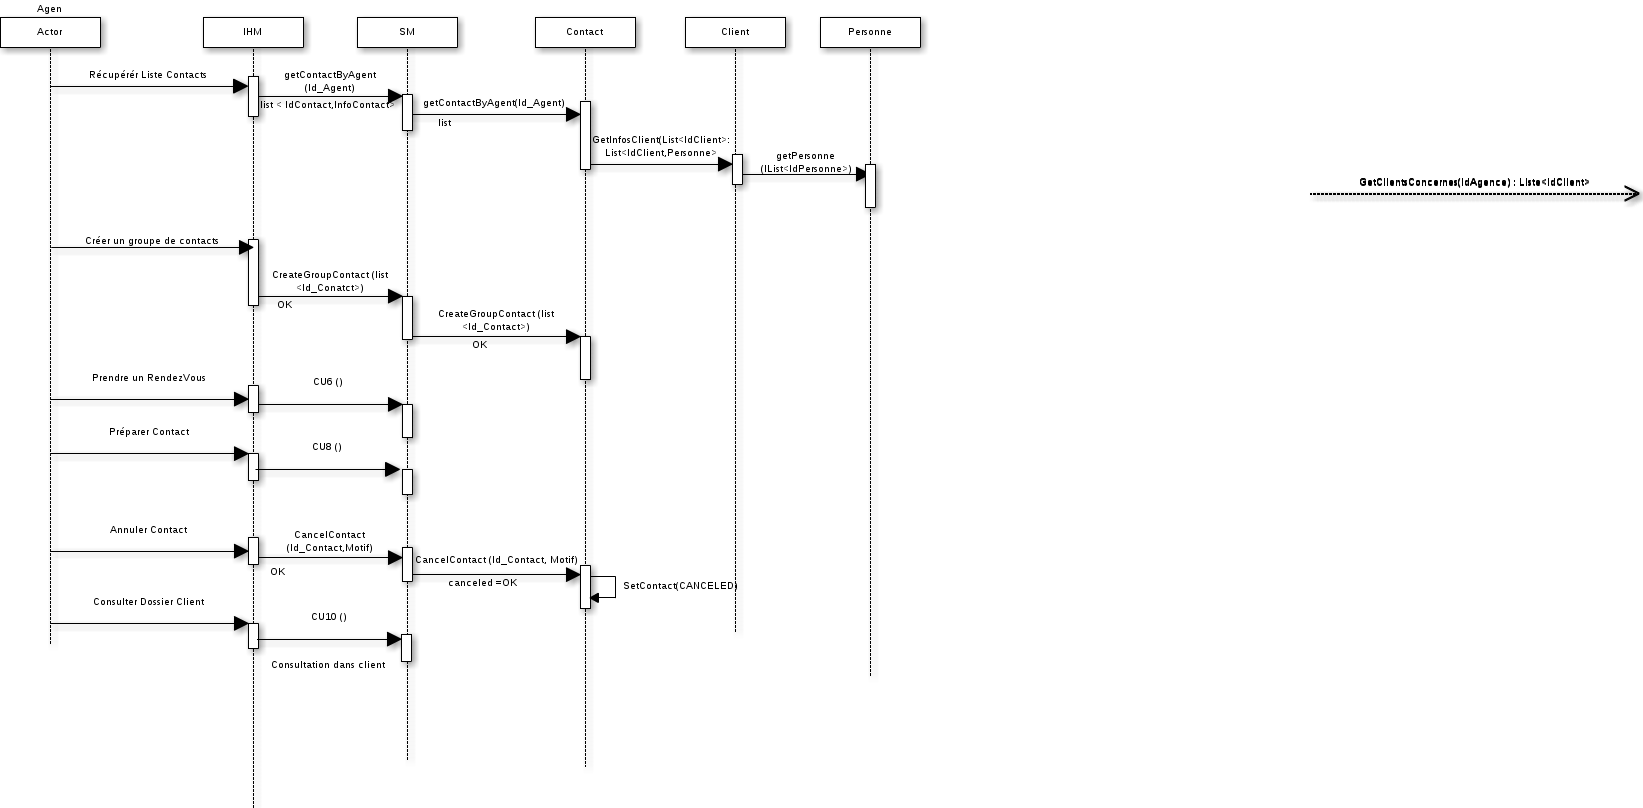
\includegraphics[scale=0.4]{Includes/SOA-Sequence-CU4.png}
		\caption{Diagramme de séquence pour le CU4}
	\end{center}
\end{figure}

\begin{figure}[H]
	\begin{center}
		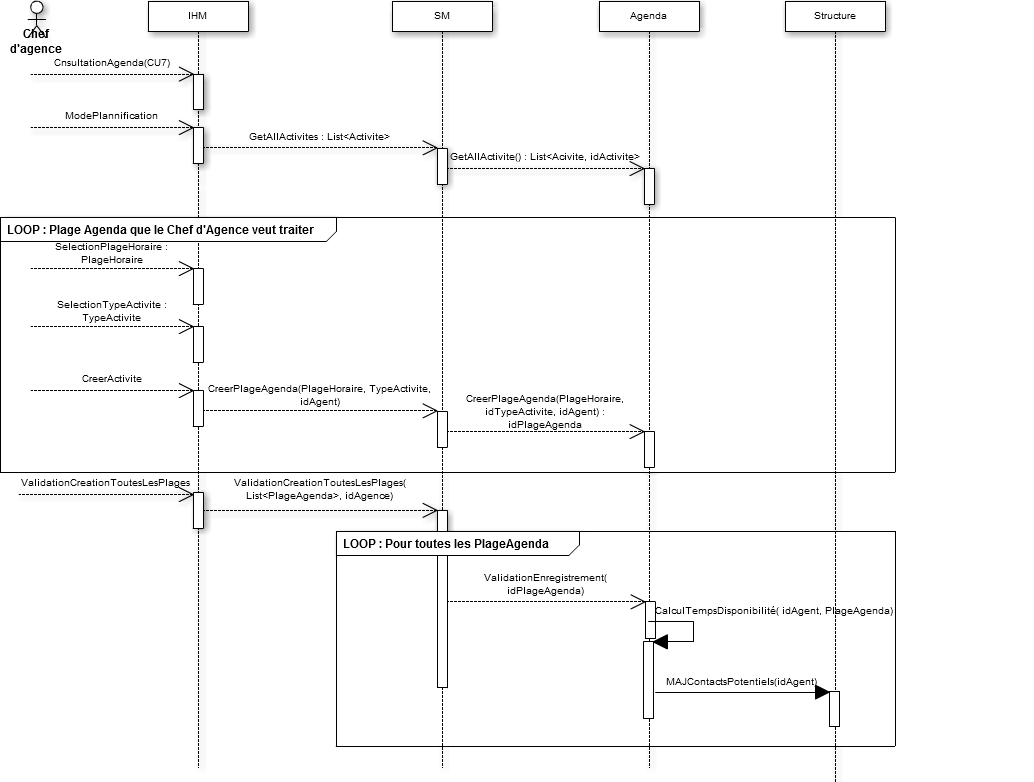
\includegraphics[scale=0.4]{Includes/SOA-Sequence-CU5.png}
		\caption{Diagramme de séquence pour le CU5}
	\end{center}
\end{figure}



\begin{figure}[H]
	\begin{center}
		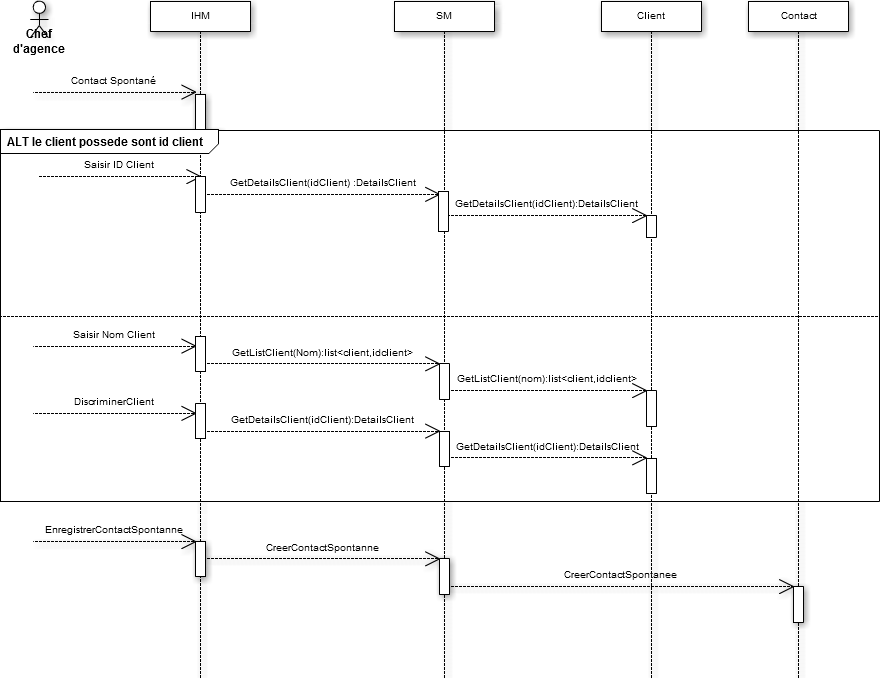
\includegraphics[scale=0.4]{Includes/SOA-Sequence-CU6-a.png}
		\caption{Diagramme de séquence pour le CU6-a}
	\end{center}
\end{figure}
\begin{figure}[H]
	\begin{center}
		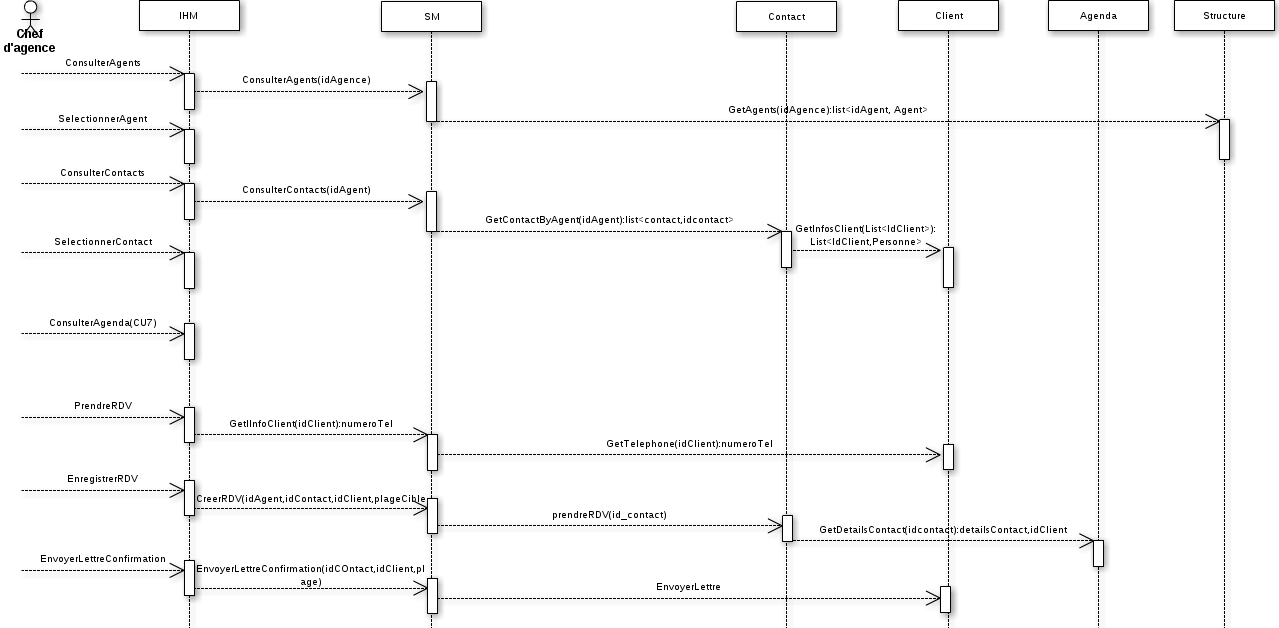
\includegraphics[scale=0.4]{Includes/SOA-Sequence-CU6-b.png}
		\caption{Diagramme de séquence pour le CU6-b}
	\end{center}
\end{figure}

\begin{figure}[H]
	\begin{center}
		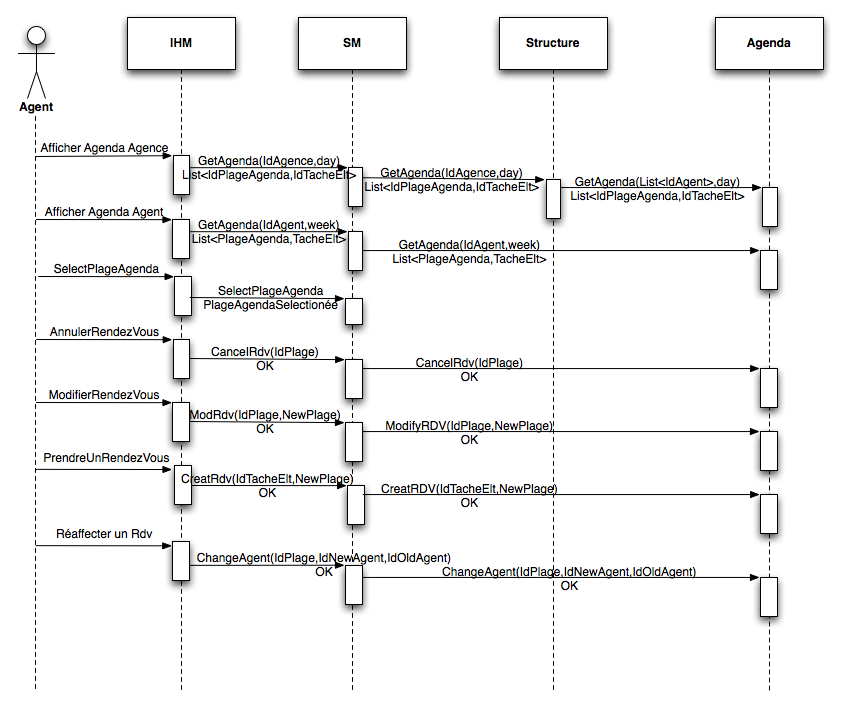
\includegraphics[scale=0.4]{Includes/SOA-Sequence-CU7.png}
		\caption{Diagramme de séquence pour le CU7}
	\end{center}
\end{figure}

\begin{figure}[H]
	\begin{center}
		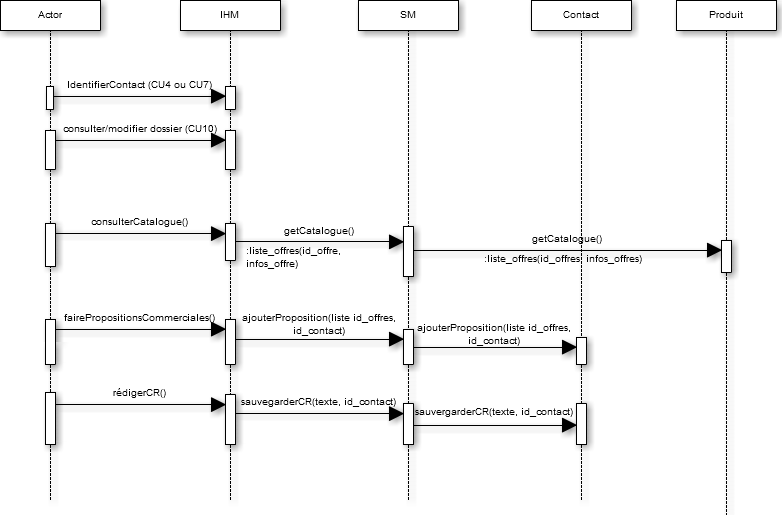
\includegraphics[scale=0.4]{Includes/SOA-Sequence-CU8.png}
		\caption{Diagramme de séquence pour le CU8}
	\end{center}
\end{figure}

\begin{figure}[H]
	\begin{center}
		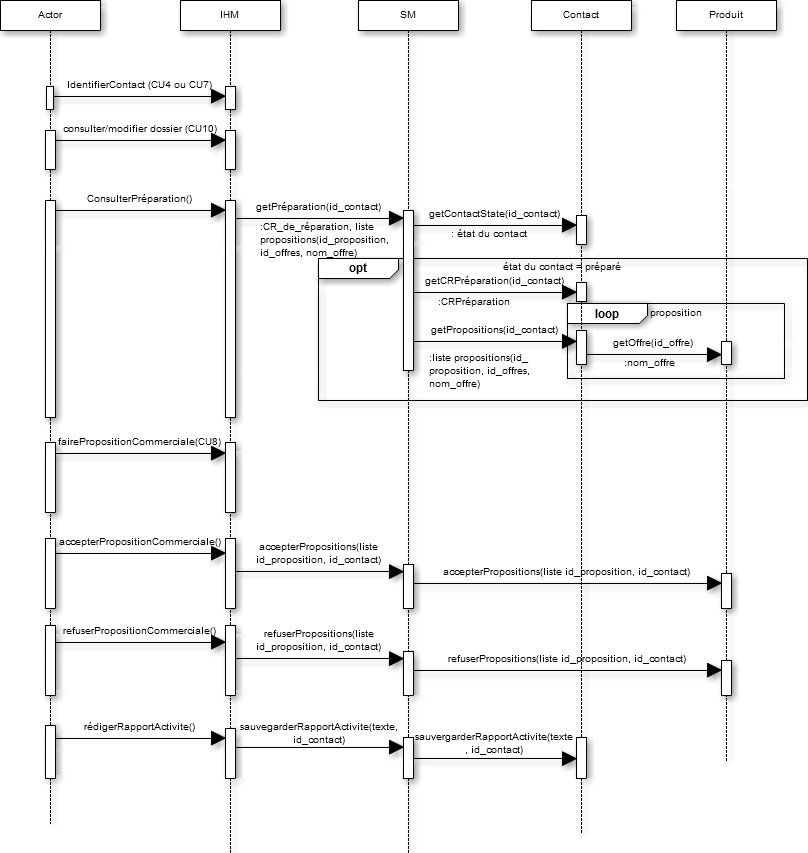
\includegraphics[scale=0.4]{Includes/SOA-Sequence-CU9.png}
		\caption{Diagramme de séquence pour le CU9}
	\end{center}
\end{figure}

\begin{figure}[H]
	\begin{center}
		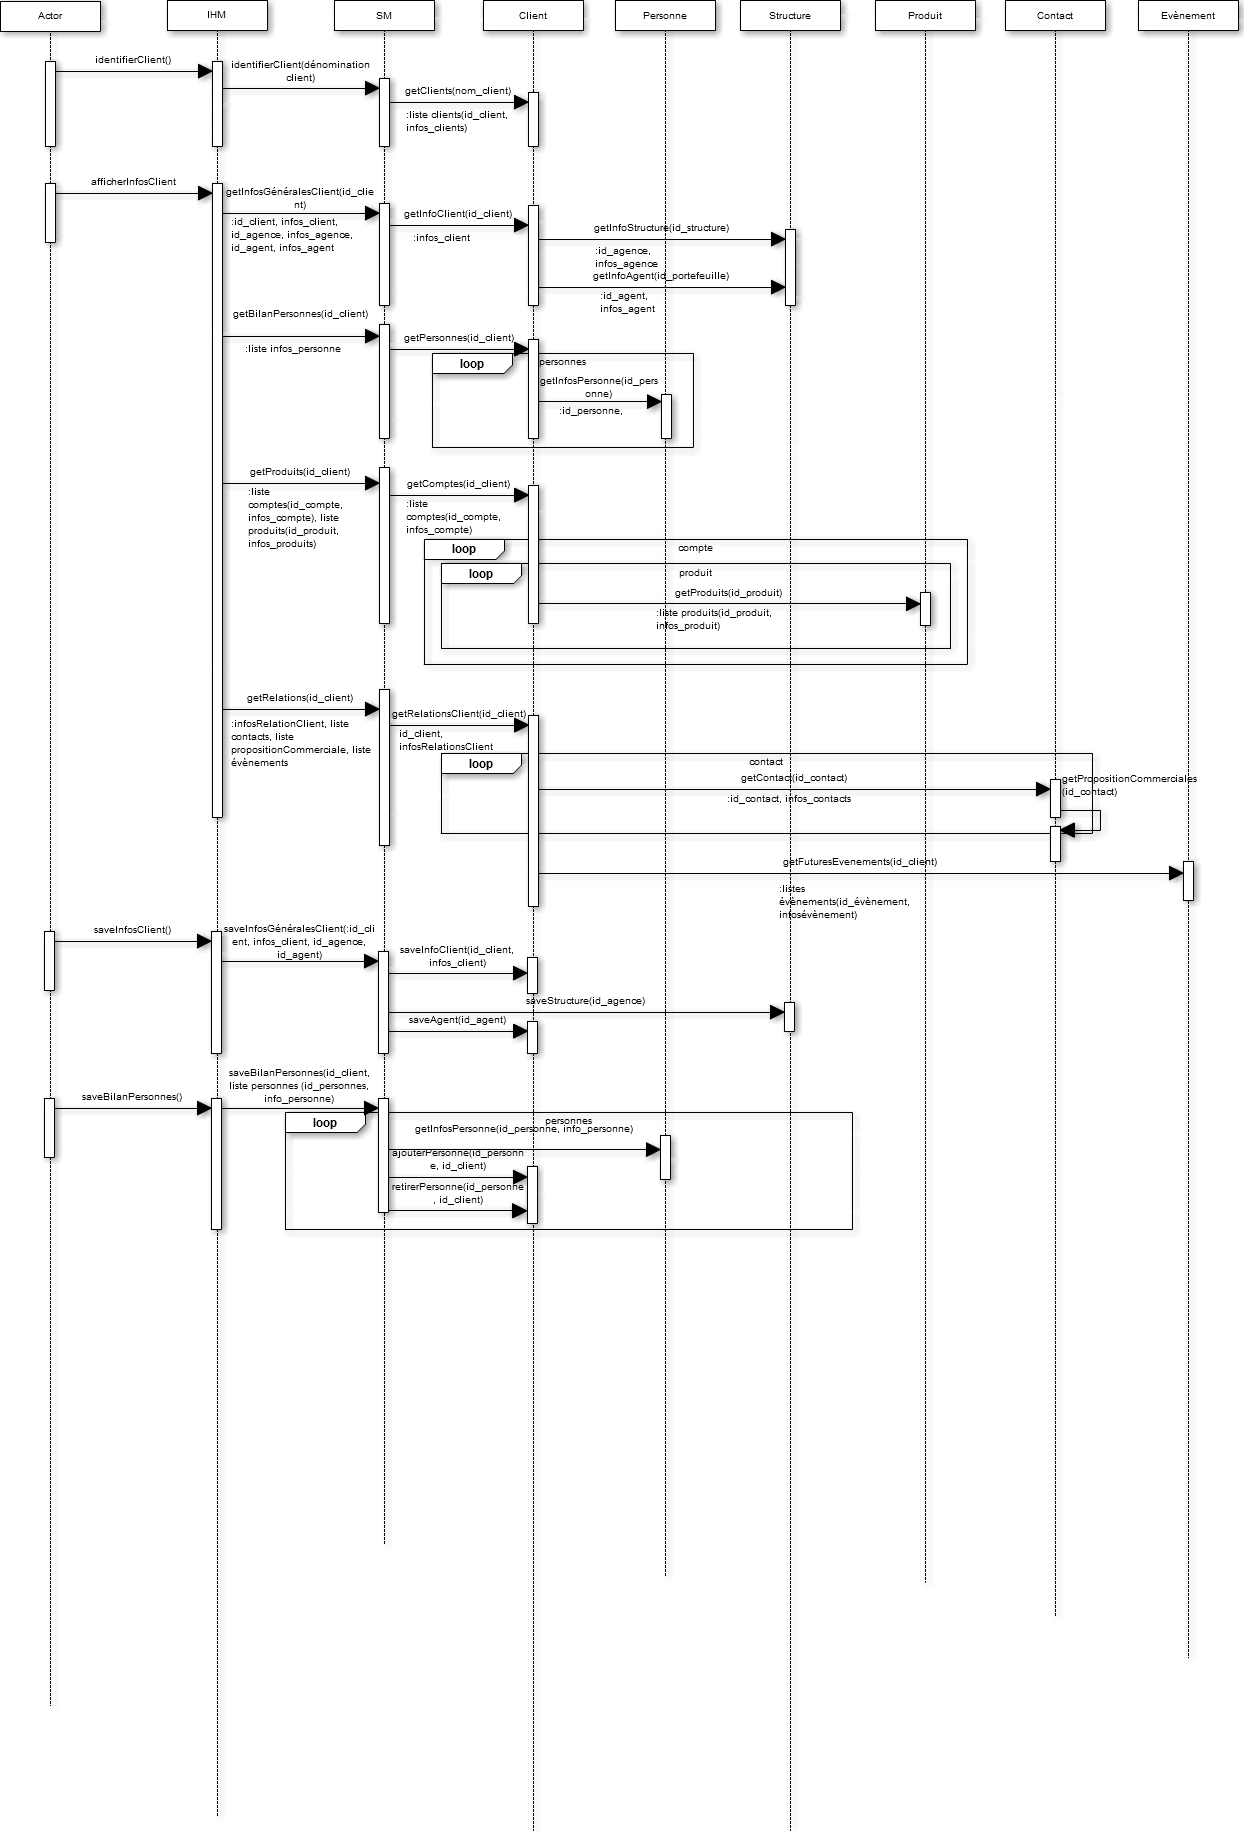
\includegraphics[scale=0.4]{Includes/SOA-Sequence-CU10.png}
		\caption{Diagramme de séquence pour le CU10}
	\end{center}
\end{figure}
